\subsubsection{User Tutorial}
In order to ensure the user fully understands how to utilize the device, a user tutorial should be provided in a similar fashion to shown in Fig. \ref{fig:user_tutorial}. Additional panels for user configuration settings should also be included for user clarity.
\begin{figure}
    \begin{subfigure}{0.5\textwidth}
        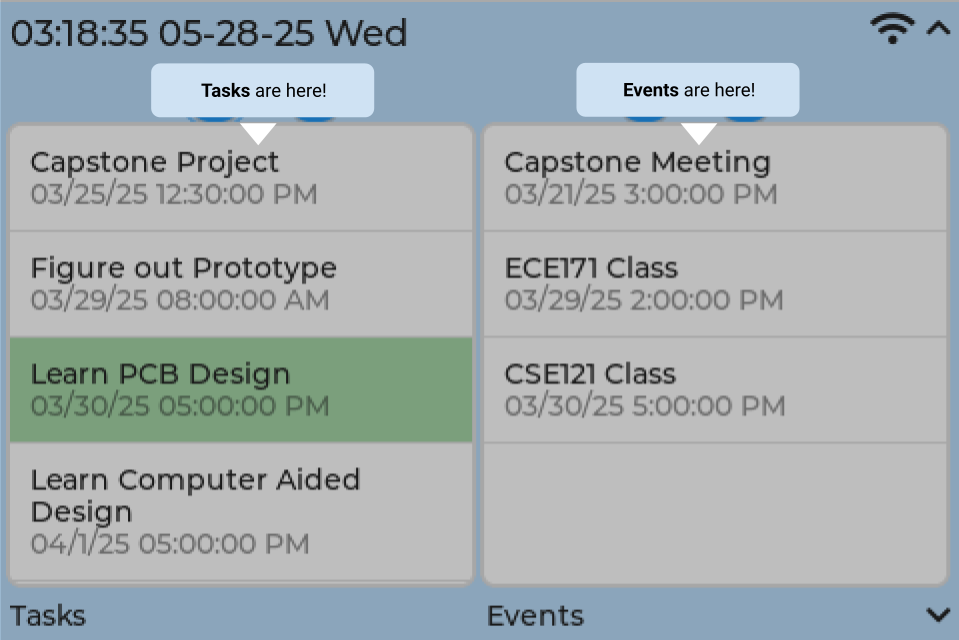
\includegraphics[width = \textwidth]{task_event.png}
        \caption{Shows what the different columns mean}
    \end{subfigure}
    \begin{subfigure}{0.5\textwidth}
        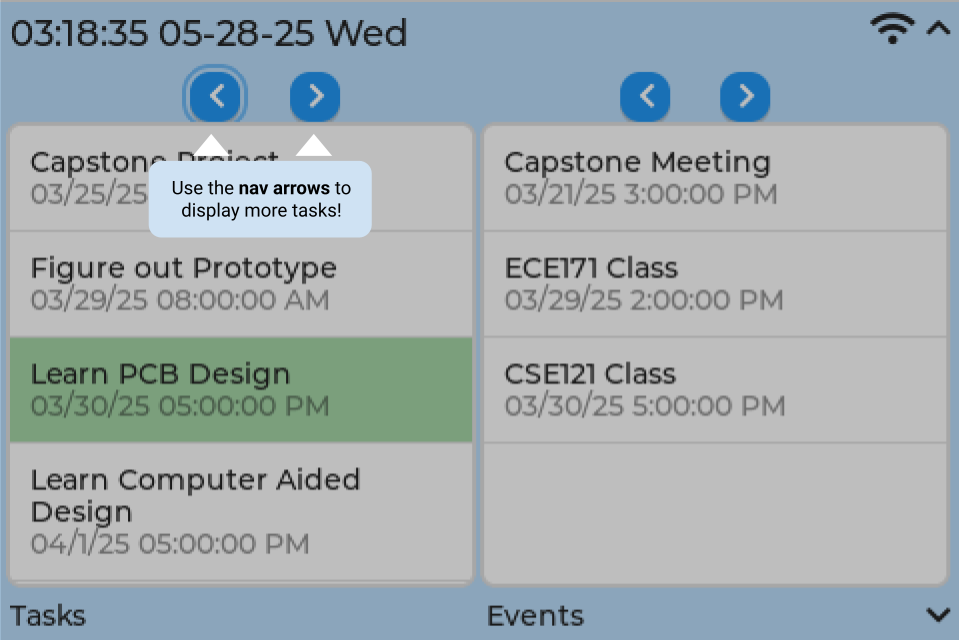
\includegraphics[width = \textwidth]{nav_arrows.png}
        \caption{Introduces navigation arrows}
    \end{subfigure}
    \begin{subfigure}{0.5\textwidth}
        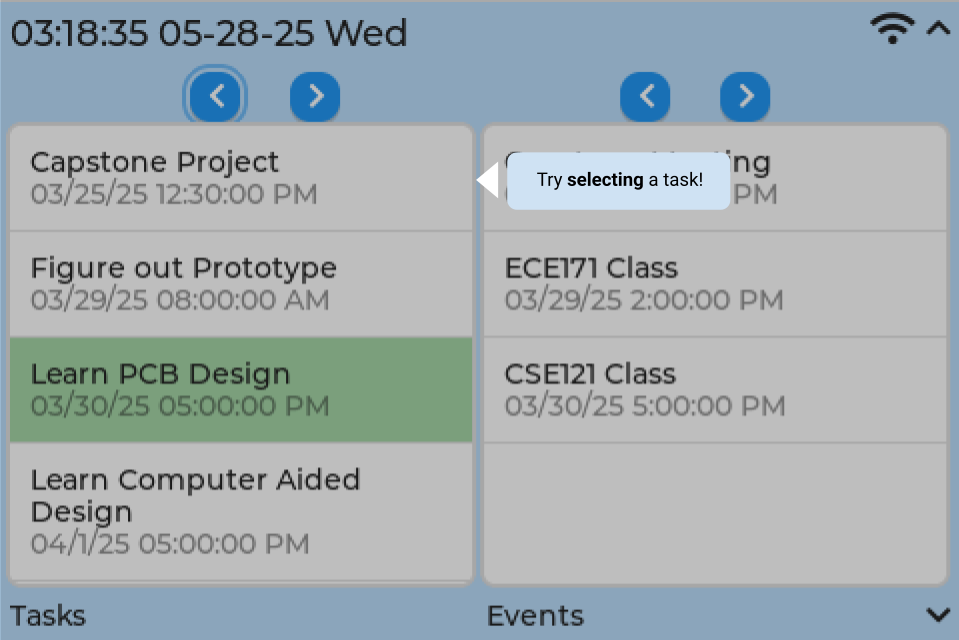
\includegraphics[width = \textwidth]{task_select.png}
        \caption{Tells user to select a task}
    \end{subfigure}
    \begin{subfigure}{0.5\textwidth}
        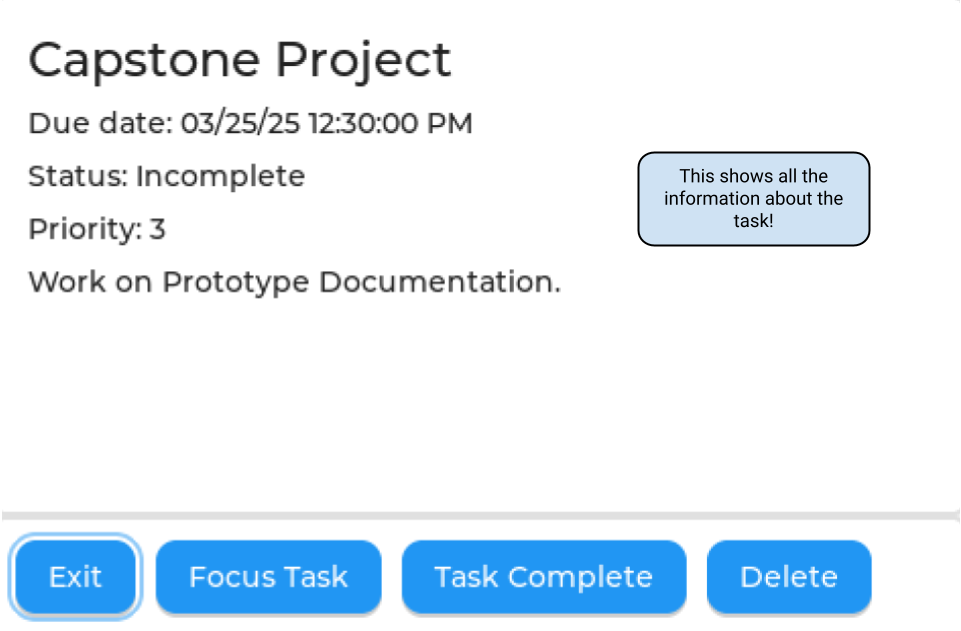
\includegraphics[width = \textwidth]{task_detail.png}
        \caption{Introduces task detail view}
    \end{subfigure}

    \begin{subfigure}{0.5\textwidth}
        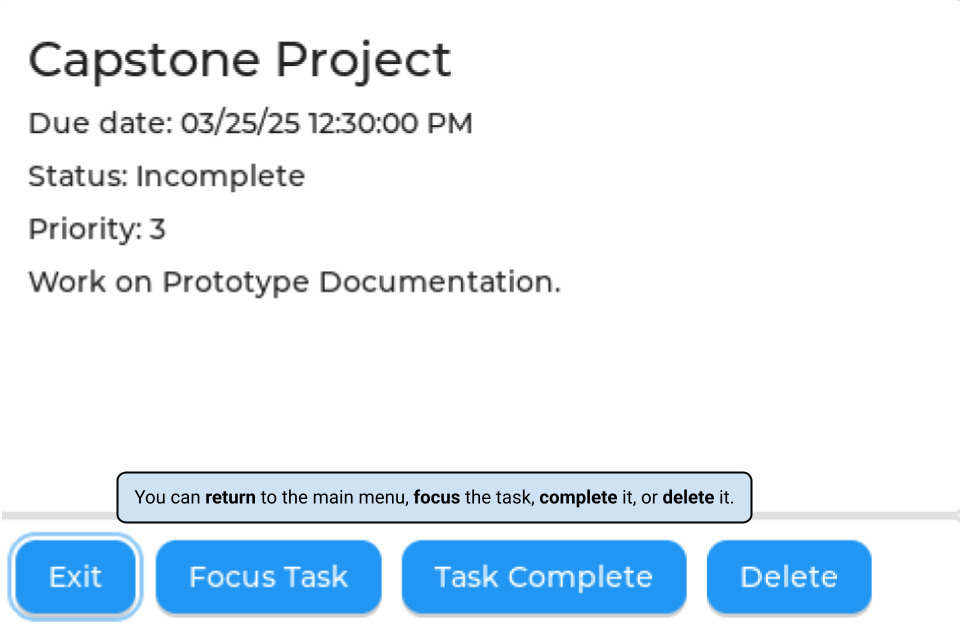
\includegraphics[width = \textwidth]{task_buttons.png}
        \caption{Introduces task interaction buttons}
    \end{subfigure}
    \begin{subfigure}{0.5\textwidth}
        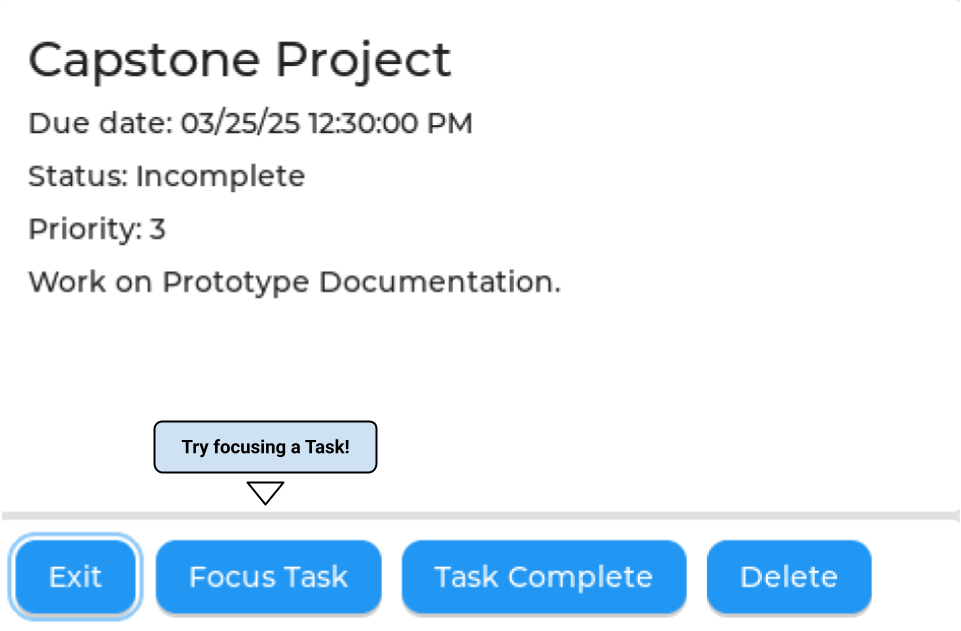
\includegraphics[width = \textwidth]{try_focus.png}
        \caption{Tells user to try focusing a task}
    \end{subfigure}
\end{figure}
\begin{figure}
    \ContinuedFloat
    \begin{subfigure}{0.5\textwidth}
        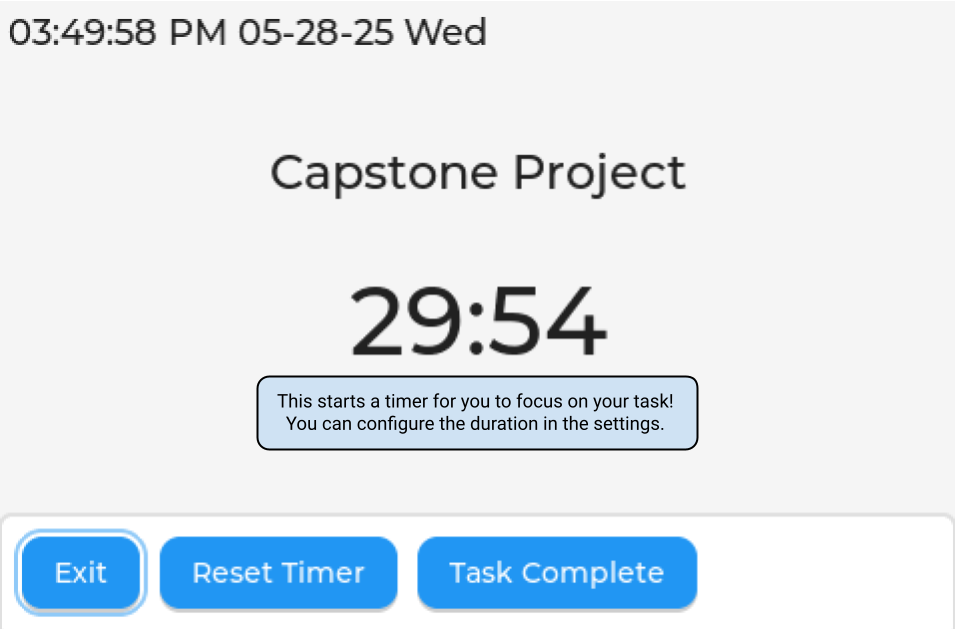
\includegraphics[width = \textwidth]{focus_tutorial.png}
        \caption{Introduces focus mode}
    \end{subfigure}
    \begin{subfigure}{0.5\textwidth}
        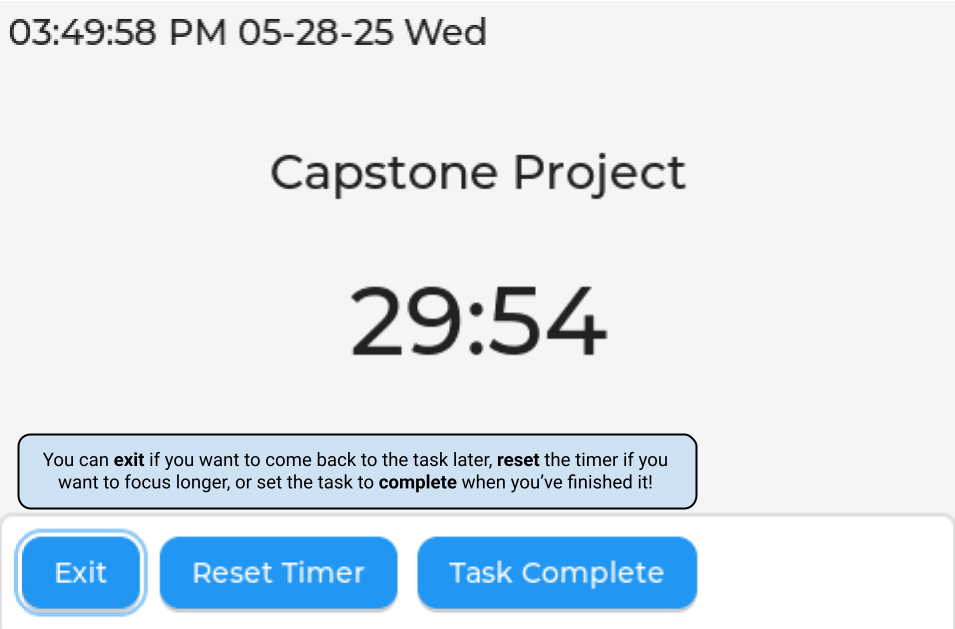
\includegraphics[width = \textwidth]{focus_buttons.png}
        \caption{Introduces focus interaction buttons}
    \end{subfigure}
    \begin{subfigure}{0.5\textwidth}
        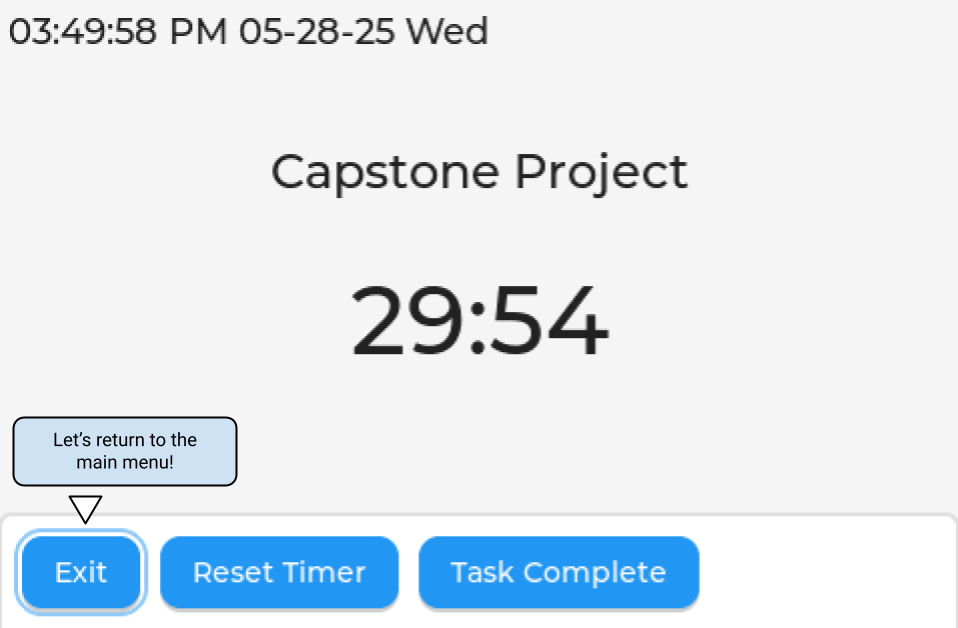
\includegraphics[width = \textwidth]{Return.png}
        \caption{Tells user to return to main menu}
    \end{subfigure}
    \begin{subfigure}{0.5\textwidth}
        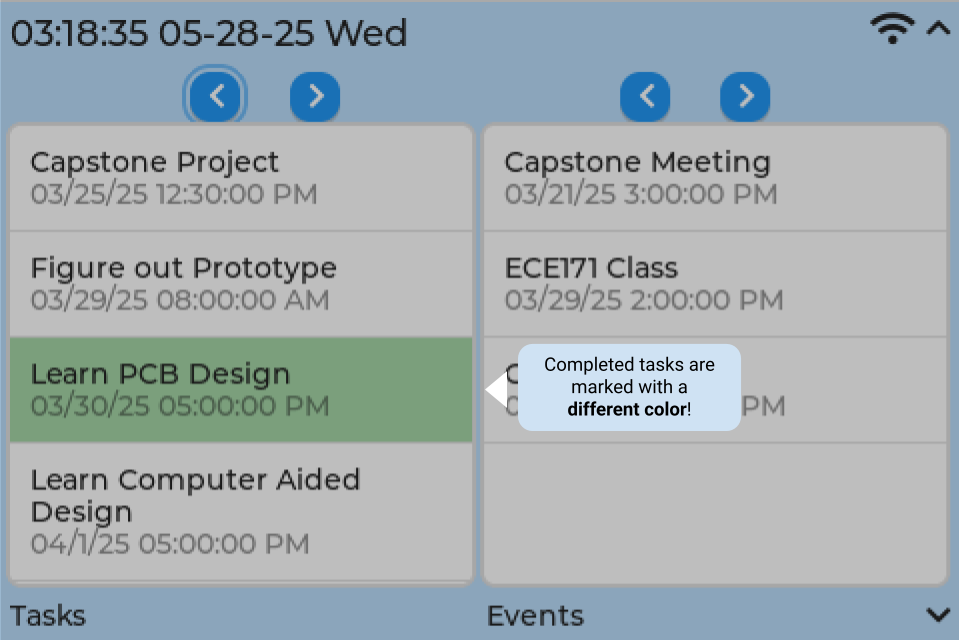
\includegraphics[width = \textwidth]{completed_task.png}
        \caption{Introduces completed tasks}
    \end{subfigure}
    \begin{subfigure}{0.5\textwidth}
        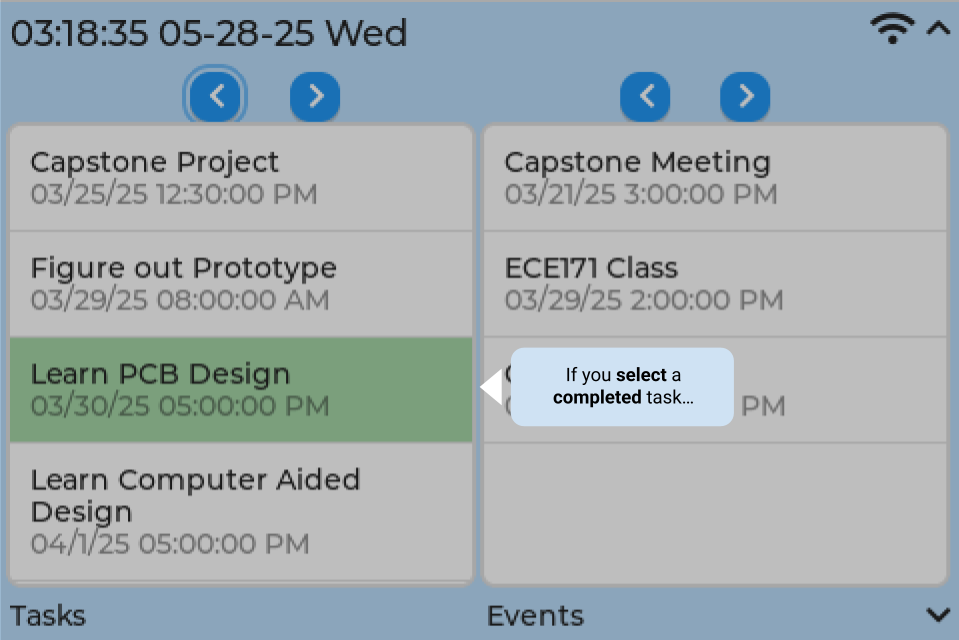
\includegraphics[width = \textwidth]{select_completed.png}
        \caption{Tells user to select completed task}
    \end{subfigure}
    \begin{subfigure}{0.5\textwidth}
        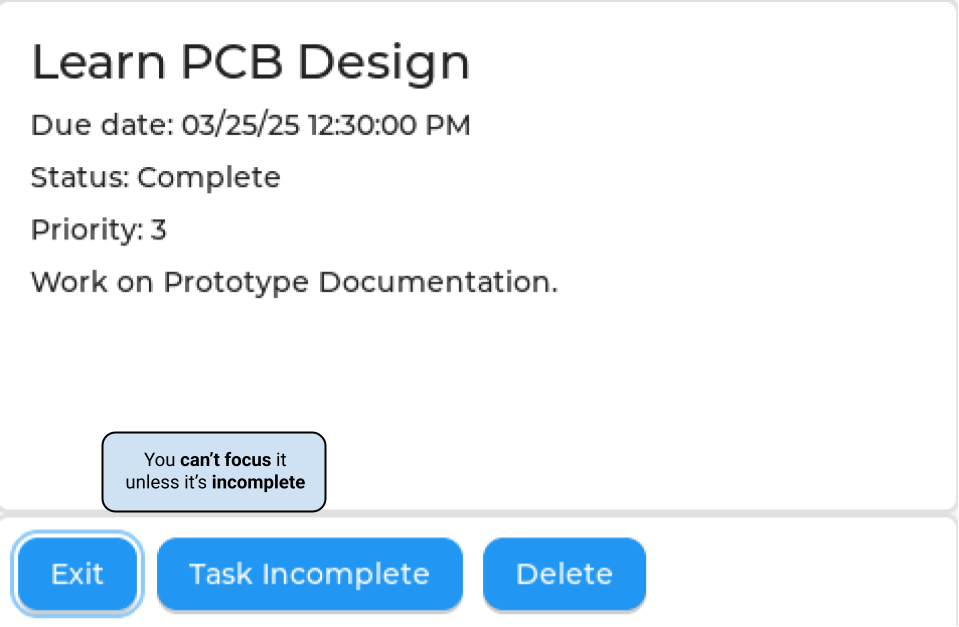
\includegraphics[width = \textwidth]{cant_focus.png}
        \caption{Informs user they cannot focus completed tasks}
    \end{subfigure}
    \end{figure}
\begin{figure}
	\ContinuedFloat
    \begin{subfigure}{0.5\textwidth}
        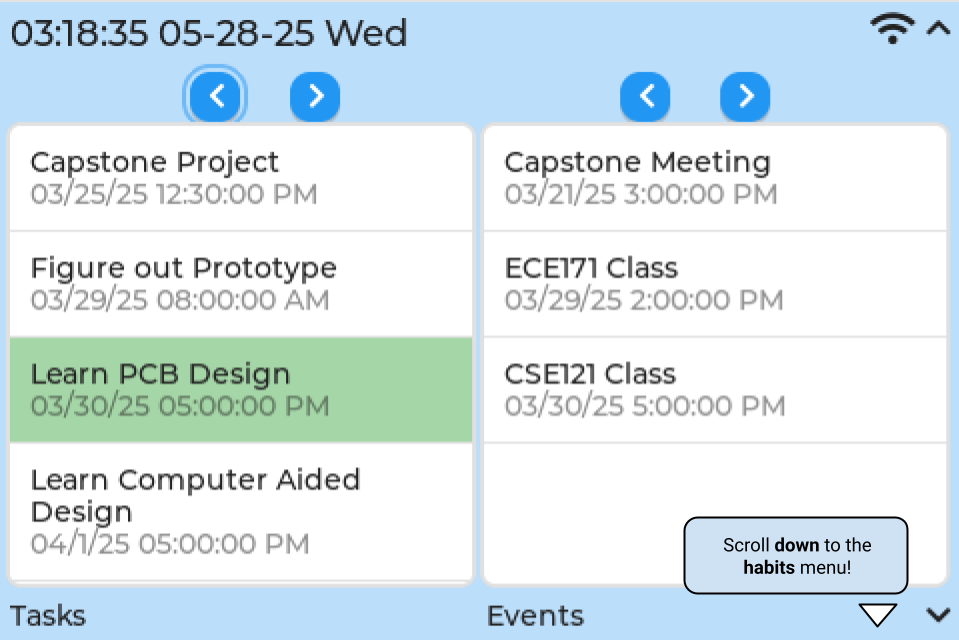
\includegraphics[width = \textwidth]{scroll_habits.png}
        \caption{Instructs user to scroll to find habits menu}
    \end{subfigure}
    \begin{subfigure}{0.5\textwidth}
        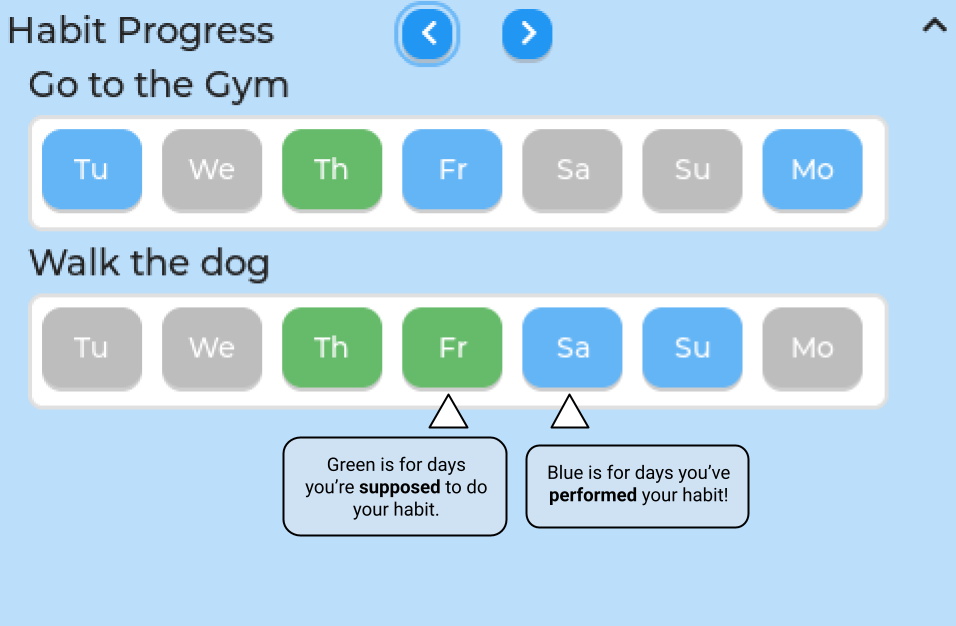
\includegraphics[width = \textwidth]{habit_tutorial.png}
        \caption{Introduces color meanings for habits}
    \end{subfigure}
\caption{User tutorial example}
\label{fig:user_tutorial}
\end{figure}
